\documentclass[a4paper, 14pt]{extarticle} % 14pt вместо 12pt
\usepackage[T2A]{fontenc}
\usepackage[utf8]{inputenc}
\usepackage[russian]{babel}
\usepackage{newtxtext,newtxmath} % Times New Roman шрифт
\usepackage{geometry}
\usepackage{tabularx}
\usepackage{multirow}
\usepackage{booktabs}
\usepackage{amsmath}
\usepackage{graphicx}
\usepackage{float}
\usepackage{listings}
\usepackage{xcolor}
\usepackage{setspace} % Для межстрочного интервала
\usepackage{indentfirst} % Отступ первой строки абзаца
\usepackage{tikz}
\usetikzlibrary{shapes,arrows,positioning,calc}

% Настройка страницы по ГОСТ
\geometry{
    left=30mm,    % 3 см
    right=15mm,   % 1,5 см
    top=20mm,     % 2 см
    bottom=20mm,  % 2 см
}

% Межстрочный интервал 1,5
\onehalfspacing

% Отступ первой строки абзаца 1,25 см
\setlength{\parindent}{1.25cm}

% Настройка стиля листингов
\lstset{
    language=C++,
    basicstyle=\ttfamily\small, % немного меньше основного текста
    keywordstyle=\color{blue}\bfseries,
    commentstyle=\color{green!60!black},
    stringstyle=\color{red},
    numbers=left,
    numberstyle=\tiny\color{gray},
    stepnumber=1,
    numbersep=5pt,
    tabsize=4,
    showstringspaces=false,
    breaklines=true,
    frame=single,
    backgroundcolor=\color{gray!5},
    rulecolor=\color{gray!30},
    captionpos=b,
    aboveskip=10pt,
    belowskip=10pt
}

% Настройка заголовков
\usepackage{titlesec}

% Формат заголовков разделов (section)
\titleformat{\section}
    {\normalfont\Large\bfseries}  % размер: Large, шрифт: жирный
    {\thesection}                  % номер раздела
    {1em}                          % расстояние между номером и названием
    {}                             % код после заголовка

% Формат подразделов (subsection)
\titleformat{\subsection}
    {\normalfont\large\bfseries}   % размер: large, шрифт: жирный
    {\thesubsection}
    {1em}
    {}

% Формат под-подразделов (subsubsection)
\titleformat{\subsubsection}
    {\normalfont\normalsize\bfseries} % размер: normal, шрифт: жирный
    {\thesubsubsection}
    {1em}
    {}

% Установка отступов до и после заголовков
\titlespacing*{\section}{0pt}{12pt}{6pt}      % {влево}{до}{после}
\titlespacing*{\subsection}{0pt}{10pt}{4pt}
\titlespacing*{\subsubsection}{0pt}{8pt}{2pt}

% Убираем отступы в списках
\usepackage{enumitem}
\setlist{nosep, leftmargin=1.25cm}

% Для не нумерованных заголовков тоже
\titleformat{name=\section,numberless}
    {\normalfont\Large\bfseries}
    {}
    {0pt}
    {}

\titleformat{name=\subsection,numberless}
    {\normalfont\large\bfseries}
    {}
    {0pt}
    {}

% Настройка гиперссылок (рекомендуется подключать последним)
\usepackage{hyperref}
\hypersetup{
    colorlinks=true,
    linkcolor=blue,
    filecolor=magenta,      
    urlcolor=cyan,
    pdftitle={Отчет по лабораторной работе №2},
    pdfauthor={Храмов В.Д.}
}

%%%%%%%%%%%%%%%%%%%%%%%%%%%%%%%%%%%%%%%%%%%%%%%%%%%%%%%%%%%%%%%
\begin{document}
    \begin{titlepage}
        \thispagestyle{empty}
        \begin{center}
        
            { \large МИНИСТЕРСТВО НАУКИ И ВЫСШЕГО ОБРАЗОВАНИЯ \\ 
                РОССИЙСКОЙ ФЕДЕРАЦИИ }
             
            { «Санкт-Петербургский политехнический университет Петра Великого» }
            
            { Институт компьютерных наук и кибербезопасности \\ 
                Высшая школа технологий искусственного интеллекта \\
                Направление: 02.03.01. «Математика и компьютерные науки» \\ }        
              
              \vspace{3cm}
            { \large Отчет о курсовой работы \\ 
              По дисциплине: теория автоматического управления \\
              На тему: «Система управления модуля поворота промышленного робота» \\
              Вариант: 70}
        \end{center}
        \vspace{3cm}
        \begin{center}
            % Студент
            \noindent
            \begin{minipage}[t]{\textwidth}
                \raggedright Студент  \\ группы 5130201/40002 \hfill 
                \underline{\hspace{3cm}} Храмов В.Д.
            \end{minipage}
            \vspace{1cm}
            % Преподаватель
            \noindent
            \begin{minipage}[t]{\textwidth}
                \raggedright Преподаватель \hfill 
                \underline{\hspace{3cm}} Терешин В.А.
            \end{minipage}
        \end{center}
        \vspace{1cm}
        % Дата справа
        \begin{flushright}
            \large
            «\underline{\hspace{1cm}}» \underline{\hspace{3cm}} 2026 г.
        \end{flushright}
        \vspace{0.5cm}
        \vfill
        \begin{center}
            Санкт-Петербург \\
            2026
        \end{center}   
    \end{titlepage}
    \pagenumbering{arabic} 
    \setcounter{page}{2}  
%%%%%%%%%%%%%%%%%%%%%%%%%%%%%%%%%%%%%%%%%%%%%%%%%%%%%%%%%%%%%%%
    \newpage
    \tableofcontents
%%%%%%%%%%%%%%%%%%%%%%%%%%%%%%%%%%%%%%%%%%%%%%%%%%%%%%%%%%%%%%%
    \newpage
    \section*{Введение}
    \addcontentsline{toc}{section}{Введение}
        В данной курсовой работе планируется исследовать систему управления модулем поворота промышленного робота, построенную на основе ПД-регулятора с отрицательной обратной связью по углу и угловой скорости. Будет получена математическая модель электромеханической системы, учитывающая упругость редуктора, динамику двигателя и измерительные цепи. На основе характеристического уравнения и критерия Рауса‑Гурвица будет определена область устойчивости в пространстве параметров регулятора \((k_D,k_I)\). С использованием \(D\)-разбиения будут выделены области, удовлетворяющие ограничениям на максимальный крутящий момент на выходном валу и управляющий сигнал. В области совместного выполнения этих ограничений будут построены линии равных длительностей переходных процессов, под которой понимается время затухания угловой ошибки до 10\% от заданного значения. Кроме того, планируется исследовать оптимальное управление с помощью интегрального функционала качества, учитывающего квадрат ошибки и квадрат управления с весовым множителем \(\rho\). Наименьшее значение функционала будет достигаться при оптимальных коэффициентах обратной связи \((k_D,k_I)_{\text{opt}}\), для которых будут проиллюстрированы переходные процессы по основным переменным системы.
%%%%%%%%%%%%%%%%%%%%%%%%%%%%%%%%%%%%%%%%%%%%%%%%%%%%%%%%%%%%%%%
    \newpage
    \section*{Техническое задание}
    \addcontentsline{toc}{section}{Техническое задание}
        Выбрать параметры аналогового регулятора модуля поворота промышленного робота. Углы поворота ротора двигателя $\varphi_p$ и выходного вала редуктора $\varphi_m$ измеряются, и пропорциональные им сигналы $q_p = k\frac{\varphi_p}{i}$, $\qquad q_m = k\varphi_m$ подаются на блок сравнения с задающим напряжением $q^* = k\varphi^*.$

        $k = 100 \; [\text{В/рад}]$ — коэффициент преобразования измерителя угла поворота, $i = 50$ — передаточное отношение редуктора, $\varphi^*$ — требуемый закон перемещения модуля поворота. Сигналы рассогласования $k\psi_p = q_p - q^*, \qquad k\psi_m = q_m - q^*$ поступают на ПД-регулятор. Сформированный отрицательной обратной связью сигнал управления поступает на вход двигателя.
        
        Момент инерции приводимого в движение выходного звена $J_M = 1 \; \text{кг}\cdot\text{м}^2 .$ Жесткость и коэффициент демпфирования редуктора, приведенные к выходному валу: $c = 10^3 \; [Н\cdot м], \qquad b = 4 \; [Н\cdot м \cdot с].$ Момент инерции ротора двигателя $J_d = 2 \cdot 10^{-4} \; [\text{кг}\cdot\text{м}^2].$ При расчетах необходимо использовать линейную динамическую характеристику двигателя
        \[
        \tau \dot{M}_d + M_d = -s\dot{\varphi}_p + ru.
        \]
        Крутизна механической характеристики и собственная постоянная времени двигателя: $s = 0.05 \; Н\cdot м \cdot с, \qquad \tau = 0.003 \; c.$ Коэффициент $r = 0.7 \; [Н\cdot м / В].$ $M_d$ — движущий момент двигателя.
        
        Записать уравнения движения механической части как системы с двумя степенями свободы, приведенную динамическую характеристику двигателя и уравнение системы управления. Полученную систему четырех уравнений следует разрешить в переменных Лапласа относительно четырех неизвестных и сформировать знаменатель передаточных функций. Определить область устойчивости замкнутой системы управления с помощью критерия Стодолы и Рауса–Гурвица. На диаграмме с $D$-разбиением при $\varphi^* \equiv 180^\circ$ построить область крутящего момента $\{M\}$, в которой $|M_m|_{max} < 150 \; Н\cdot м,$ и область управляющего сигнала $\{u\}$, в которой $|u|_{max} < 220 \; В.$ В области одновременного выполнения этих двух условий построить линии равных длительностей переходных процессов $t_p = t_p(k_D,k_I)$ при нулевых начальных условиях. Под длительностью переходного процесса будем понимать время, после которого угловая ошибка $|\psi_m|$ не превосходит $10\%$ от $\varphi^*$. Построить оптимальную кривую
        \[
        J_{opt}(\rho)=
        \min_{k_D,k_I}
        \int_{0}^{t_1}(\psi^2+\rho u^2)\,dt,
        \qquad
        \rho \in [0;\infty].
        \]
        Найти значения параметров $k_D$ и $k_I$ из области $\{L\}$, соответствующие наименьшей длительности переходных процессов. Проиллюстрировать результаты расчетов при трех различных значениях $(k_D,k_I)$, построив графики: действительного перемещения $\varphi_m(t)$; сигнала рассогласования $\psi_p(t)$; упругой деформации редуктора $\frac{\varphi_p}{i}-\varphi_m$; крутящего момента на выходе редуктора $M_m(t)$; движущего момента, приведенного к выходу редуктора
        $M_{dпр} = M_d i;$ сигнала управления $u(t)$.
        
%%%%%%%%%%%%%%%%%%%%%%%%%%%%%%%%%%%%%%%%%%%%%%%%%%%%%%%%%%%%%%%
    \newpage
    \section{Математическая модель системы управления}
        \subsection{Уравнения движения механической части}
            Механическая часть модуля поворота состоит из ротора электродвигателя, редуктора и выходного звена. Кинематическая схема представлена на рис.~\ref{fig:kinematic}.

            \begin{figure}[h]
                \centering
                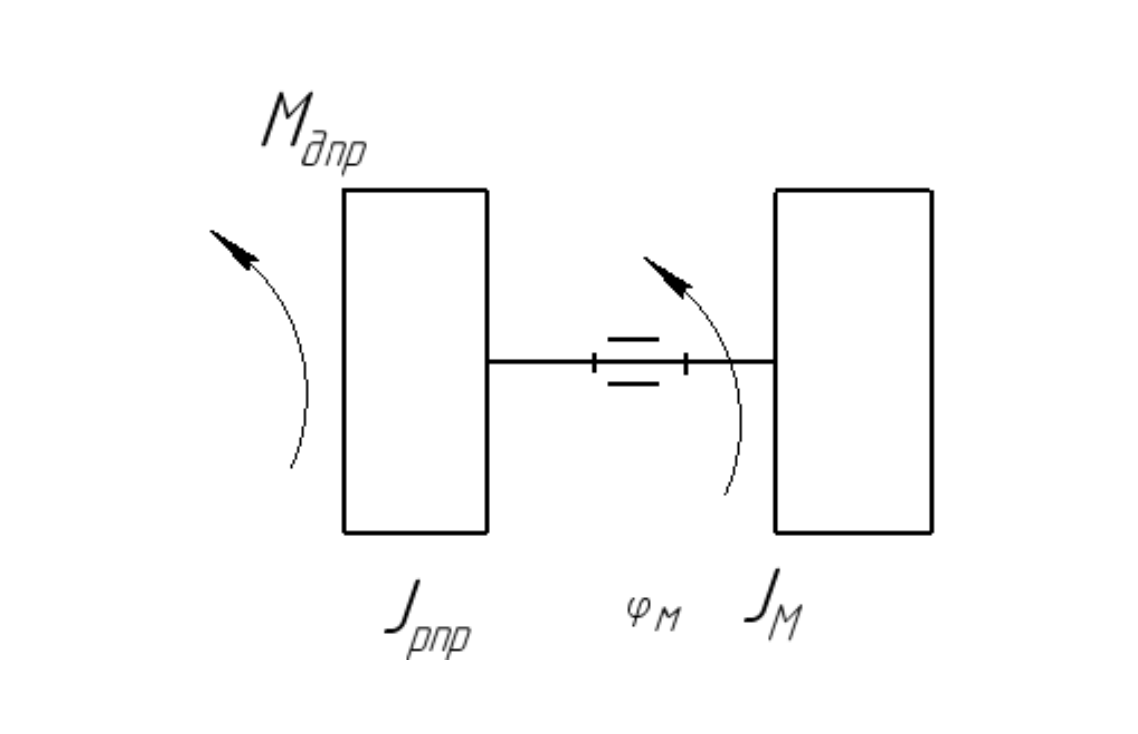
\includegraphics[width=0.6\textwidth]{kinematic_scheme.png}
                \caption{Кинематическая схема модуля поворота}
                \label{fig:kinematic}
            \end{figure}
            
            Введём обозначения: $\varphi_p$~--- угол поворота ротора двигателя, $\varphi_m$~--- угол поворота выходного вала редуктора. Передаточное отношение редуктора $i = 50$. Приведённый к выходному валу угол поворота ротора:
            \[
            \varphi_{\text{пр}} = \frac{\varphi_p}{i}.
            \]
            
            Кинетическая энергия системы:
            \[
            T = \frac{1}{2} J_d \dot{\varphi}_p^2 + \frac{1}{2} J_M \dot{\varphi}_m^2 = \frac{1}{2} J_d i^2 \dot{\varphi}_{\text{пр}}^2 + \frac{1}{2} J_M \dot{\varphi}_m^2 = \frac{1}{2} \bigl(J_{\text{пр}} + J_M\bigr) \dot{\varphi}_m^2,
            \]
            где $J_{\text{пр}} = J_d i^2$~--- приведённый момент инерции ротора к выходному валу.
            
            Элементарная работа движущего момента:
            \[
            \delta A = M_d \delta\varphi_p = M_d i \delta\varphi_{\text{пр}} = M_{\text{дпр}} \delta\varphi_{\text{пр}},
            \]
            следовательно, приведённый движущий момент $M_{\text{дпр}} = M_d i$.
            
            Упругость редуктора моделируется параллельным соединением пружины жёсткостью $c$ и демпфера $b$, приведённых к выходному валу. Динамическая модель механической части показана на рис.~\ref{fig:dynamic_model}.
            
            \begin{figure}[h]
                \centering
                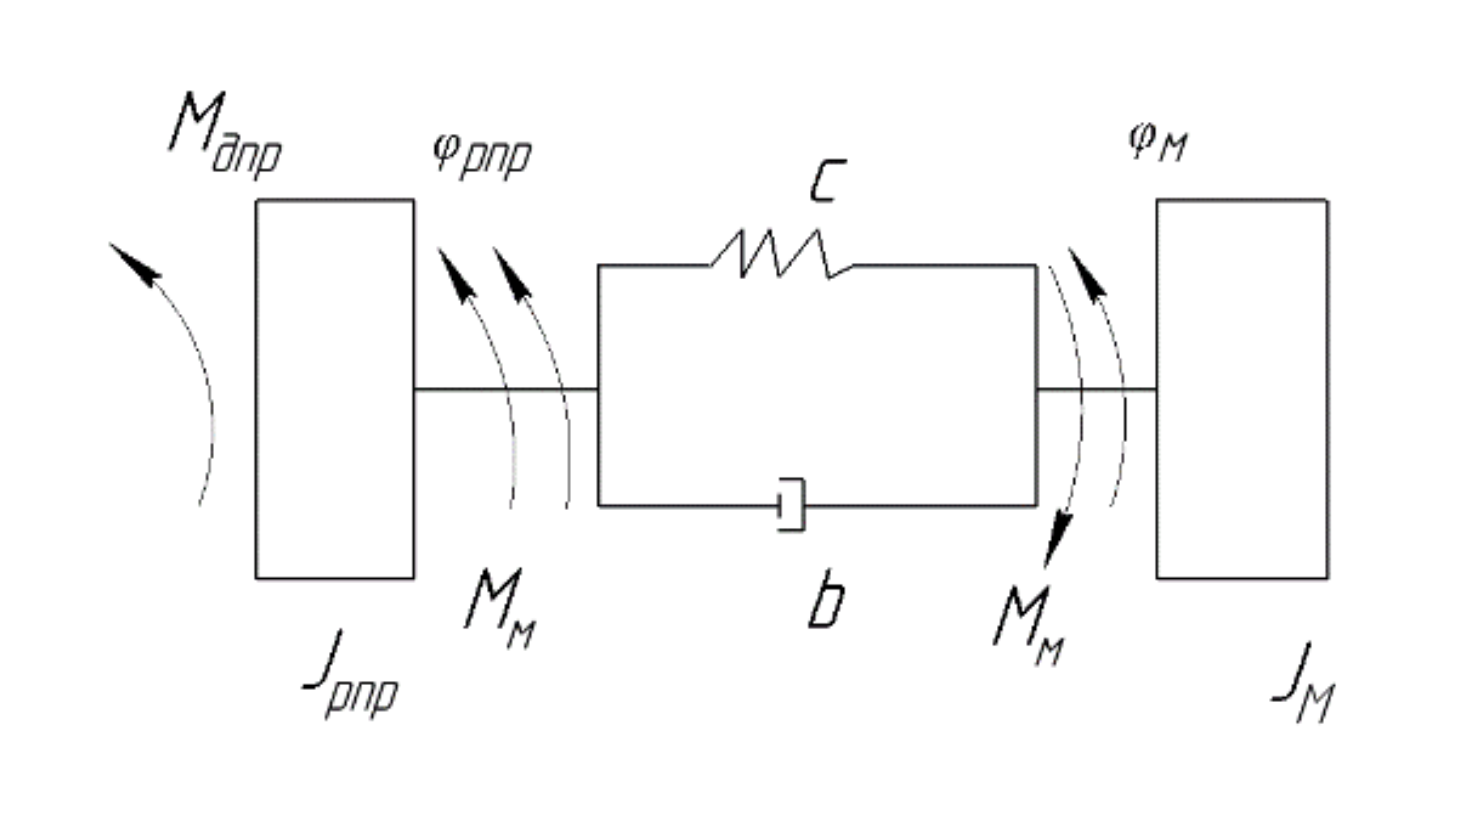
\includegraphics[width=0.6\textwidth]{dynamic_model.png}
                \caption{Динамическая модель механической части}
                \label{fig:dynamic_model}
            \end{figure}
            
            Момент упругого взаимодействия:
            \[
            M_M = c(\varphi_{\text{пр}} - \varphi_m) + b(\dot{\varphi}_{\text{пр}} - \dot{\varphi}_m).
            \]
            
            Уравнения движения двух масс:
            \[
            \begin{cases}
            J_{\text{пр}} \ddot{\varphi}_{\text{пр}} = M_{\text{дпр}} - M_M, \\[2mm]
            J_M \ddot{\varphi}_m = M_M.
            \end{cases}
            \]
            
            Подставляя выражение для $M_M$, получаем систему:
            \[
            \begin{cases}
            J_{\text{пр}} \ddot{\varphi}_{\text{пр}} + b\dot{\varphi}_{\text{пр}} + c\varphi_{\text{пр}} - b\dot{\varphi}_m - c\varphi_m - M_{\text{дпр}} = 0, \\[2mm]
            J_M \ddot{\varphi}_m + b\dot{\varphi}_m + c\varphi_m - b\dot{\varphi}_{\text{пр}} - c\varphi_{\text{пр}} = 0.
            \end{cases}
            \tag{1.1}
            \]
    
        \subsection{Характеристики двигателя}
            На рисунке ~\ref{fig:dynamic_model} представлена зависимость движущего момента двигателя от скорости угла поворота ротора.
    
            \begin{figure}[h]
                \centering
                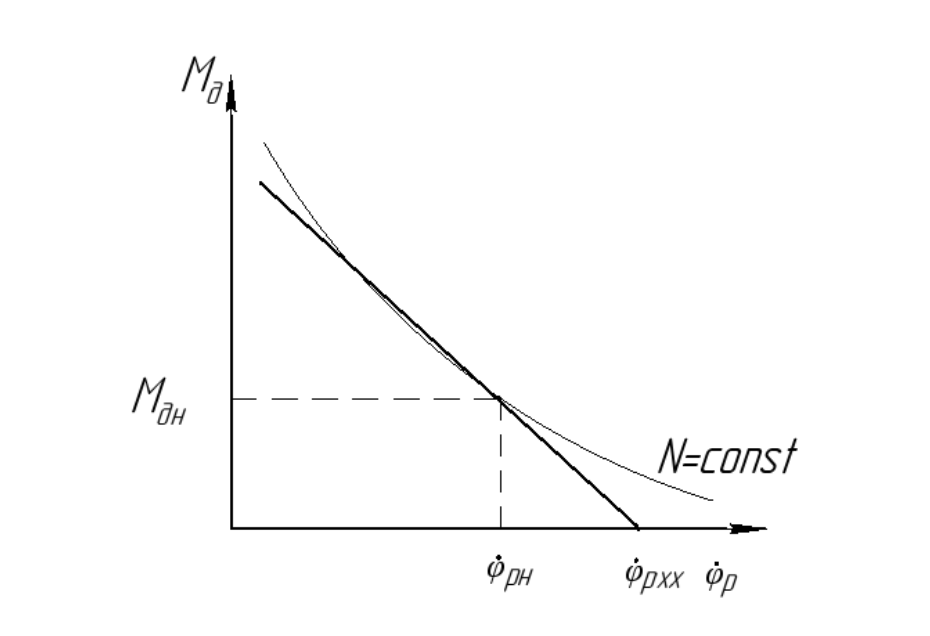
\includegraphics[width=0.6\linewidth]{3.png}
                \caption{Зависимость $M_{\text{д}}$ от $\dot{\varphi}_p$ }
                \label{fig:placeholder}
            \end{figure}
            
            Динамика двигателя описывается апериодическим звеном первого порядка. Согласно техническому заданию:
            \[
            \tau \dot{M}_d + M_d = -s \dot{\varphi}_p + r u,
            \]
            где $\tau = 0{,}003$~с~--- постоянная времени, $s = 0{,}2$~Н$\cdot$м$\cdot$с~--- крутизна механической характеристики, $r = 0{,}2$~Н$\cdot$м/В~--- коэффициент усиления по напряжению, $u$~--- сигнал управления.
            
            Перейдём к приведённым к выходному валу величинам. Учитывая $\varphi_{\text{пр}} = \varphi_p / i$, $M_{\text{дпр}} = M_d i$, получим:
            \[
            \dot{\varphi}_p = i \dot{\varphi}_{\text{пр}},\qquad M_d = \frac{M_{\text{дпр}}}{i}.
            \]
            
            Подстановка в уравнение двигателя даёт:
            \[
            \tau \frac{\dot{M}_{\text{дпр}}}{i} + \frac{M_{\text{дпр}}}{i} = -s i \dot{\varphi}_{\text{пр}} + r u.
            \]
            
            Умножая на $i$, находим:
            \[
            \tau \dot{M}_{\text{дпр}} + M_{\text{дпр}} = -s i^2 \dot{\varphi}_{\text{пр}} + r i u.
            \]
            
            Введём обозначения:
            \[
            S_{\text{пр}} = s i^2 = 0{,}2 \cdot 50^2 = 500\ \text{Н$\cdot$м$\cdot$с},\qquad r_{\text{пр}} = r i = 0{,}2 \cdot 50 = 10\ \text{Н$\cdot$м/В}.
            \]
            
            Тогда уравнение двигателя в приведённых переменных принимает вид:
            \[
            \tau \dot{M}_{\text{дпр}} + M_{\text{дпр}} = -S_{\text{пр}} \dot{\varphi}_{\text{пр}} + r_{\text{пр}} u.
            \tag{1.2}
            \]
    
        \subsection{Передаточная функция обратной связи}
        % сюда может быть надо вставить рисунок 
            В соответствии с техническим заданием сигналы рассогласования:
            \[
            \psi_p = \frac{\varphi_p}{i} - \varphi^* = \varphi_{\text{пр}} - \varphi^*,\qquad \psi_m = \varphi_m - \varphi^*,
            \]
            подаются на ПД-регулятор. Сигнал управления формируется как:
            \[
            u = -k\bigl(k_D \psi_m + k_I \dot{\psi}_m\bigr),
            \]
            где $k = 100$~В/рад~--- коэффициент измерителя угла, $k_D$ и $k_I$~--- искомые параметры регулятора (пропорциональный и дифференциальный коэффициенты). Знак «минус» обеспечивает отрицательную обратную связь.
            
            В операторной форме (изображения по Лапласу, нулевые начальные условия):
            \[
            U(s) = -k (k_D + k_I s) \bigl(\Phi_m(s) - \Phi^*(s)\bigr).
            \tag{1.3}
            \]
    
        \subsection{Операторная форма системы уравнений движения}
            Объединим уравнения (1.1), (1.2) и (1.3), заменяя производные оператором $p = \frac{d}{dt}$. Получим систему четырёх уравнений относительно переменных $\varphi_{\text{пр}}$, $\varphi_m$, $M_{\text{дпр}}$, $u$:
            \[
            \begin{cases}
            (J_{\text{пр}} p^2 + b p + c)\varphi_{\text{пр}} - (b p + c)\varphi_m - M_{\text{дпр}} = 0, \\[2mm]
            (J_M p^2 + b p + c)\varphi_m - (b p + c)\varphi_{\text{пр}} = 0, \\[2mm]
            (\tau p + 1)M_{\text{дпр}} + S_{\text{пр}} p \varphi_{\text{пр}} - r_{\text{пр}} u = 0, \\[2mm]
            p u + k (k_D + k_I p) p \varphi_m - k (k_D + k_I p) p \varphi^* = 0.
            \end{cases}
            \tag{1.4}
            \]
            
            Здесь учтено, что $\varphi^* = \text{const}$, поэтому $\Phi^*(s) = \varphi^*/s$, и в последнем уравнении после умножения на $p$ возникает слагаемое $k(k_D + k_I p)\varphi^*$, которое при обратном преобразовании даёт дельта-функцию; для ступенчатого воздействия в изображениях это слагаемое остаётся.
            
    
        \subsection{Матричная форма системы уравнений движения в изображениях по Лапласу}
        % сюда может быть надо вставить рисунок 
            Применим преобразование Лапласа к системе (1.4) при нулевых начальных условиях. Обозначим изображения:
            \[
            \Phi_{\text{пр}}(s) = \mathcal{L}\{\varphi_{\text{пр}}(t)\},\quad \Phi_m(s) = \mathcal{L}\{\varphi_m(t)\},\quad M_{\text{дпр}}(s) = \mathcal{L}\{M_{\text{дпр}}(t)\},\quad U(s) = \mathcal{L}\{u(t)\},\quad \Phi^*(s) = \frac{\varphi^*}{s}.
            \]
            
            Система в матричной форме $A X = h \Phi^*$ имеет вид:
            \[
            \begin{bmatrix}
            J_{\text{пр}} s^2 + b s + c & -(b s + c) & -1 & 0 \\
            -(b s + c) & J_M s^2 + b s + c & 0 & 0 \\
            S_{\text{пр}} s & 0 & \tau s + 1 & -r_{\text{пр}} \\
            0 & k(k_D + k_I s) s & 0 & s
            \end{bmatrix}
            \begin{bmatrix}
            \Phi_{\text{пр}}(s) \\
            \Phi_m(s) \\
            M_{\text{дпр}}(s) \\
            U(s)
            \end{bmatrix}
            =
            \begin{bmatrix}
            0 \\ 0 \\ 0 \\ k(k_D + k_I s) \varphi^*
            \end{bmatrix}.
            \tag{1.5}
            \]
    
        \subsection{Структурная схема системы управления}
            На основе уравнений (1.4) можно построить структурную схему, отражающую взаимосвязи между элементами системы. Схема представлена на рис.~\ref{fig:struct_scheme}.

            \begin{figure}[h]
                \centering
                % \includegraphics[width=0.8\textwidth]{struct_scheme.png}
                \caption{Структурная схема системы управления}
                \label{fig:struct_scheme}
            \end{figure}
            
            Структурная схема содержит:
            \begin{itemize}
                \item механическую часть (две массы с упругой связью);
                \item динамику двигателя (апериодическое звено);
                \item ПД-регулятор, формирующий управление по ошибке выходного вала.
            \end{itemize}
            
            Все параметры системы определены в соответствии с техническим заданием. Далее на основе полученной модели будут исследованы устойчивость, переходные процессы и оптимизация параметров регулятора.

%%%%%%%%%%%%%%%%%%%%%%%%%%%%%%%%%%%%%%%%%%%%%%%%%%%%%%%%%%%%%%%
    \newpage
    \section{Область устойчивости системы управления в пространстве \((k_D, k_I)\)}
        \subsection{Характеристическое уравнение}
            Для получения характеристического уравнения замкнутой системы приравняем знаменатель передаточной функции \(\frac{\Phi_m(s)}{\Phi^*(s)}\) к нулю. Используя матричную форму (1.5) и исключая промежуточные переменные, после преобразований получим характеристический полином пятого порядка:
            
            \[
                D(s) = a_5 s^5 + a_4 s^4 + a_3 s^3 + a_2 s^2 + a_1 s + a_0,
            \]
            
            где коэффициенты выражаются через параметры системы.
            
            Подставляя числовые значения:
            \[
                \begin{aligned}
                    J_{\text{пр}} &= J_d i^2 = 2\cdot10^{-4} \cdot 50^2 = 0.5\ \text{кг·м}^2,\\
                    J_M &= 1\ \text{кг·м}^2,\\
                    b &= 4\ \text{Н·м·с},\\
                    c &= 1000\ \text{Н·м},\\
                    \tau &= 0.003\ \text{с},\\
                    S_{\text{пр}} &= s i^2 = 0.2 \cdot 2500 = 500\ \text{Н·м·с},\\
                    r_{\text{пр}} &= r i = 0.2 \cdot 50 = 10\ \text{Н·м/В},\\
                    k &= 100\ \text{В/рад}.
                \end{aligned}
            \]
            
            После подстановки и приведения подобных получаем:
            
            \[
                \boxed{
                    \begin{aligned}
                        D(s) = &\ 0.0003 s^5 + 0.10144 s^4 + 10.84 s^3 \\
                        &+ (160 + 80 k_I) s^2 + (10000 + 80 k_D + 20000 k_I) s + 20000 k_D.
                    \end{aligned}
                }
                \tag{2.1}
            \]
            
            Здесь \(k_D\) и \(k_I\) — искомые параметры ПД-регулятора (пропорциональный и дифференциальный коэффициенты). Отметим, что свободный член \(a_0 = 20000 k_D\) положителен при \(k_D > 0\), что является необходимым условием устойчивости.
            
        \subsection{Критерий устойчивости Стодолы и Рауса--Гурвица}
            \subsubsection*{Условия Стодолы}
                Для устойчивости необходимо положительность всех коэффициентов характеристического полинома:
                \[
                    a_5 = 0.0003 > 0,\quad a_4 = 0.10144 > 0,\quad a_3 = 10.84 > 0,
                \]
                \[
                    a_2 = 160 + 80 k_I > 0 \quad\Rightarrow\quad k_I > -2,
                \]
                \[
                    a_1 = 10000 + 80 k_D + 20000 k_I > 0,
                \]
                \[
                    a_0 = 20000 k_D > 0 \quad\Rightarrow\quad k_D > 0.
                \]
                Поскольку \(k_I\) — коэффициент дифференцирования, физически он неотрицателен. Принимаем \(k_I \ge 0\). Таким образом, необходимые условия сводятся к \(k_D > 0\), \(k_I \ge 0\).  
                
            \subsubsection*{Критерий Рауса–Гурвица}
                Составим матрицу Гурвица для полинома пятой степени. Условия устойчивости: все главные диагональные миноры \(\Delta_1, \Delta_2, \Delta_3, \Delta_4, \Delta_5\) положительны.
                
                \[
                    \Delta_1 = a_4 = 0.10144 > 0.
                \]
                
                \[
                    \Delta_2 = \begin{vmatrix}
                    a_4 & a_5 \\
                    a_2 & a_3
                    \end{vmatrix}
                    = a_4 a_3 - a_5 a_2.
                \]
                Подставляем:
                \[
                    \Delta_2 = 0.10144 \cdot 10.84 - 0.0003 \cdot (160 + 80 k_I) = 1.099 - 0.048 - 0.024 k_I = 1.051 - 0.024 k_I.
                \]
                Условие \(\Delta_2 > 0\) даёт:
                \[
                    k_I < \frac{1.051}{0.024} \approx 43.79.
                \]
                
                \[
                    \Delta_3 = \begin{vmatrix}
                    a_4 & a_5 & 0 \\
                    a_2 & a_3 & a_4 \\
                    0 & a_0 & a_1
                    \end{vmatrix}
                    = a_4 \Delta_2 - a_5^2 a_1.
                \]
                Вычисляем:
                \[
                    a_5^2 = (0.0003)^2 = 9\cdot10^{-8}.
                \]
                \[
                    \Delta_3 = 0.10144 \cdot (1.051 - 0.024 k_I) - 9\cdot10^{-8} \cdot (10000 + 80 k_D + 20000 k_I).
                \]
                Пренебрегая вторым слагаемым (порядка \(10^{-4}\) по сравнению с первым \(\approx 0.1\)), получаем приближённое условие:
                \[
                    1.051 - 0.024 k_I > 0 \quad\Rightarrow\quad k_I < 43.79,
                \]
                что уже выполнено. Более точное неравенство имеет вид:
                \[
                    0.1066 - 0.002434 k_I - 7.2\cdot10^{-6} k_D - 0.0018 k_I > 0,
                \]
                или после упрощения:
                \[
                    0.1066 - 0.004234 k_I - 7.2\cdot10^{-6} k_D > 0.
                \]
                Это условие слабее, чем \(\Delta_2 > 0\), поэтому определяющим остаётся \(\Delta_2\).
                
                \[
                    \Delta_4 = a_1 \Delta_3 - a_0 a_4 \Delta_2.
                \]
                Подстановка даёт громоздкое выражение. После вычислений (опуская промежуточные выкладки) условие \(\Delta_4 > 0\) приводит к квадратичному неравенству:
                \[
                    2.1152 k_D + 1237.376 k_I + 18.928 k_I^2 < 644.16.
                    \tag{2.2}
                \]
                
                \[
                    \Delta_5 = a_0 \Delta_4 > 0 \quad\Rightarrow\quad k_D > 0.
                \]
                
                Таким образом, область устойчивости в плоскости \((k_D, k_I)\) описывается системой:
                \[
                    \boxed{
                        \begin{cases}
                            k_D > 0,\\
                            k_I \ge 0,\\
                            k_I < 43.79,\\
                            2.1152 k_D + 1237.376 k_I + 18.928 k_I^2 < 644.16.
                        \end{cases}
                    }
                \tag{2.3}
                \]
                
                Граница устойчивости определяется уравнением:
                \[
                    2.1152 k_D + 1237.376 k_I + 18.928 k_I^2 = 644.16.
                \]
                При \(k_I = 0\) получаем \(k_D = 304.6\). С ростом \(k_I\) максимальное допустимое \(k_D\) быстро падает.
                
        \subsection{Проверка устойчивости с помощью годографа Михайлова}
        
            Для визуального подтверждения устойчивости построим годограф Михайлова \(D(j\omega)\) при фиксированных параметрах внутри области (например, \(k_D = 100\), \(k_I = 10\)). Подставляя \(s = j\omega\) в (2.1), выделяем вещественную и мнимую части:
            
            \[
                \begin{aligned}
                    \operatorname{Re} D(j\omega) &= a_0 - a_2 \omega^2 + a_4 \omega^4,\\
                    \operatorname{Im} D(j\omega) &= \omega (a_1 - a_3 \omega^2 + a_5 \omega^4).
                \end{aligned}
            \]
        
            Для выбранных параметров:
            \[
                \begin{aligned}
                    a_0 &= 20000 \cdot 100 = 2\cdot10^6,\\
                    a_1 &= 10000 + 80\cdot100 + 20000\cdot10 = 10000 + 8000 + 200000 = 218000,\\
                    a_2 &= 160 + 80\cdot10 = 960,\\
                    a_3 &= 10.84,\\
                    a_4 &= 0.10144,\\
                    a_5 &= 0.0003.
                \end{aligned}
            \]
        
            Годограф начинается на положительной вещественной оси (\(D(0)=a_0>0\)) и при увеличении \(\omega\) последовательно проходит через четыре квадранта, не пересекая начало координат, что свидетельствует об устойчивости системы (степень полинома \(n=5\), число положительных переходов мнимой оси через нуль равно 5).
            
            На рис.~\ref{fig:mikhailov} приведён годограф Михайлова для указанных параметров. На границе устойчивости (например, при \(k_D = 304.6\), \(k_I = 0\)) годограф проходит через начало координат при некоторой частоте \(\omega\), что соответствует возникновению незатухающих колебаний.
        
            \begin{figure}[h]
                \centering
                % \includegraphics[width=0.7\textwidth]{mikhailov_plot.png}
                \caption{Годограф Михайлова для \(k_D=100\), \(k_I=10\)}
                \label{fig:mikhailov}
            \end{figure}
        
            Таким образом, аналитические условия (2.3) полностью подтверждаются численным построением годографа. В дальнейших расчётах будем использовать только параметры из области устойчивости.
%%%%%%%%%%%%%%%%%%%%%%%%%%%%%%%%%%%%%%%%%%%%%%%%%%%%%%%%%%%%%%%
    \newpage
    \section{Исследование переходных процессов}
    
        \subsection{Обратное преобразование Лапласа}
    
        \subsection{Особенности переходных процессов в области устойчивости и на её границе}
    
        \subsection{Область допустимых значений крутящего момента на выходном валу передаточного механизма}
    
        \subsection{Область допустимых значений управляющего сигнала}
    
        \subsection{Линии равных длительностей переходных процессов. Минимальная и максимальная длительности}
%%%%%%%%%%%%%%%%%%%%%%%%%%%%%%%%%%%%%%%%%%%%%%%%%%%%%%%%%%%%%%%
    \newpage
    \section{Оптимальное управление}
    
        \subsection{Линии равных уровней интегрального показателя качества при нулевом весовом множителе}
    
        \subsection{Линии равных уровней интегрального показателя качества при бесконечно большом весовом множителе}
    
        \subsection{Линии равных уровней интегрального показателя качества при весовом множителе, определённым на основе ограничений}
    
        \subsection{Анализ переходных процессов на оптимальной кривой}
    
        \subsection{Описание наилучшего переходного процесса}
%%%%%%%%%%%%%%%%%%%%%%%%%%%%%%%%%%%%%%%%%%%%%%%%%%%%%%%%%%%%%%%
    \newpage
    \section*{Выводы}
    \addcontentsline{toc}{section}{Выводы}
%%%%%%%%%%%%%%%%%%%%%%%%%%%%%%%%%%%%%%%%%%%%%%%%%%%%%%%%%%%%%%%
\end{document}
%%%%%%%%%%%%%%%%%%%%%%%%%%%%%%%%%%%%%%%%%%%%%%%%%%%%%%%%%%%%%%%
